% !Mode:: "TeX:UTF-8"
% VL 10, gebaut aus part-representation-learning/18-rnn.md und 19-transformer.md
% (2025 war das auf VL 9 und VL 10 verteilt; Dialogmuster:
%  transcripts/vl09-representation-learning-2025 und vl10-faltung-cnn-2025).
% !Mode:: "TeX:UTF-8"
\newcommand{\thepage}{} % to silence a hyperref warning about pdfpagelabels
\RequirePackage[]{silence}
\WarningsOff[hyperref]
\PassOptionsToPackage{log-declarations=false}{xparse}
%\RequirePackage[l2tabu, orthodox]{nag}
\RequirePackage{luatex85} % to make \pdf...= commands work with LuaTeX
\documentclass[aspectratio=169,t]{beamer}
\usepackage{ifthen}
\usepackage[T1]{fontenc}
\usepackage{iftex}
\ifLuaTeX
 \usepackage{fontspec}
 \setmainfont[Ligatures=TeX]{Source Sans Pro}
\else
 \usepackage[utf8]{inputenc}
\fi
\usepackage{german}
\usepackage{newunicodechar}
\newunicodechar{€}{\texteuro}
\newunicodechar{ß}{\ss}
\renewcommand{\SS}{\iffontchar\font"1E9E \symbol{"1E9E}\else SS\fi}
\usepackage{ellipsis}
\usepackage{microtype}
\usepackage{listings}
\usepackage{sourcecodepro}
\lstset{language=Python, basicstyle=\ttfamily}
\usepackage{amsfonts}
\usepackage{amssymb}
\usepackage{amsthm}
\usepackage{fancyhdr}
\usepackage{graphicx}

\newtheorem{proposition}[theorem]{Proposition}

\DeclareMathOperator*{\argmax}{argmax}
\DeclareMathOperator{\supp}{supp}
\newcommand{\E}{\ensuremath{\mathbb{E}}}
\newcommand{\V}{\ensuremath{\mathbb{V}}}

\setbeamercolor{emph}{fg=purple}
\renewcommand<>{\emph}[1]{%
  {\usebeamercolor[fg]{emph}\only#2{\itshape}#1}%
}



\hypersetup{draft=false,colorlinks=false,pdfpagemode=UseOutlines,plainpages=false,
            breaklinks=true,bookmarksnumbered=true,pdfborder=0 0 0,
            pdftitle={Einführung in Deep Learning WiSe 2026/27 HHU},
            pdfauthor={Konrad Voelkel},
            pdfsubject={data science}}

%\documentclass[aspectratio=169,t]{beamer}
\usetheme{hhubeamer} % put the hhu-beamer-theme in /usr/share/texmf/tex/latex/beamer/themes/

% -------------------- Code listings config --------------------
% Define custom colors for syntax highlighting
\definecolor{codegreen}{rgb}{0,0.6,0}
\definecolor{codegray}{rgb}{0.5,0.5,0.5}
\definecolor{codepurple}{rgb}{0.58,0,0.82}
\definecolor{backcolour}{rgb}{0.96,0.96,0.94} % Very light gray/beige
% Configure the listings package
\lstset{
    language=Python,
    backgroundcolor=\color{backcolour},   
    commentstyle=\color{codegreen}\itshape,
    keywordstyle=\color{blue}\bfseries,
    numberstyle=\tiny\color{codegray},
    stringstyle=\color{codepurple},
    basicstyle=\ttfamily\footnotesize, % Use a monospaced font
    breakatwhitespace=false,         
    breaklines=true,      
             % Enable automatic line breaking
    captionpos=b,                      % Caption at the bottom
    keepspaces=true,                 
    numbers=left,                      % Line numbers on the left
    numbersep=10pt,                    % Distance of line numbers from the code
    showspaces=false,                
    showstringspaces=false,            % Don't show weird underscores in strings
    showtabs=false,                  
    tabsize=4,
    frame=single,                      % Add a subtle border around the code
    rulecolor=\color{black!20},        % Border color
  }

\event[]{}
\author[Wintersemester 2026/27]{Dr. Konrad Völkel, Wintersemester 2026/27}

%\title{Data Science, VL 1}
%\date{16.04.2026}


%%% Local Variables:
%%% mode: latex
%%% TeX-master: t
%%% End:


% Fassung mit Dozentennotizen (zweiter Schirm): die nächste Zeile einkommentieren.
% \setbeameroption{show notes on second screen=right}

\graphicspath{{../images/}}

\title[RNNs und Transformer (VL 10)]{RNNs und Transformer\\\large Einführung in Deep Learning, VL 10}
\date{16.12.2026}

\begin{document}

\begin{frame}
  \titlepage

  \note{\textbf{Ablauf, 90 Minuten.} 2025 war der Transformer ein Nachtrag am Anfang von
    VL 10 (22 Min.) plus 7 Min. am Ende von VL 9 --- dieses Jahr gehört ihm die halbe
    Sitzung:\\[2pt]
    \begin{tabular}{@{}rll@{}}
      0--6   & Folie 2       & Sequenzen: was ist neu?\\
      6--18  & Folien 3--4   & RNN, entfaltet, backpropagation through time\\
      18--26 & Folien 5--6   & Verschwindende Gradienten, Skip Connections\\
      26--38 & Folien 7--9   & GRU und LSTM, Code\\
      38--46 & Folie 10      & BLEU: wie misst man Übersetzung?\\
      46--60 & Folien 11--13 & \textbf{Attention}, Positionskodierung\\
      60--72 & Folien 14--15 & GPT, BPE\\
      72--84 & Folien 16--17 & BERT, ViT\\
      84--90 & Folie 18      & Letzte Sitzung vor Weihnachten, Übungsblatt\\
    \end{tabular}\\[4pt]
    \textbf{Letzte Sitzung vor der Winterpause} --- das Übungsblatt hat bis 13.01. Zeit,
    das ausdrücklich ansagen.}
\end{frame}

\begin{frame}
  \frametitle{Was ist an Sequenzen anders?}

  \begin{center}
    \Large
    Text, Audio, Video, Zeitreihen:\\[10pt]
    die Reihenfolge trägt Bedeutung.
  \end{center}

  \bigskip
  \begin{center}
    \normalsize Ein MLP sieht immer nur einen Vektor fester Länge.
  \end{center}

  \note{Frage in den Raum: Wie würden Sie einen Satz variabler Länge in ein MLP stecken?
    Antworten sammeln (padding, Mittelwert, …) und dann zeigen, dass die Reihenfolge dabei
    verloren geht --- „Katze isst Maus“ aus der letzten Woche.}
\end{frame}

\begin{frame}
  \frametitle{Die Idee des RNN}

  \begin{center}
    \Large
    $h_t = \tau(W x_t + U h_{t-1} + b)$, \qquad $y_t = V h_t$
  \end{center}

  \bigskip
  \begin{center}
    \normalsize Der Zustand von gestern geht in die Rechnung von heute ein.
  \end{center}

  \note{Drei Matrizen: $W$ für die neue Eingabe, $U$ für den alten Zustand, $V$ für die
    Ausgabe. Mehr ist es nicht.
    Begriff: Im Gegensatz zum CNN (nächste Woche, Finite Impulse Response) ist ein RNN ein
    \emph{Infinite Impulse Response}-Signalverarbeiter --- eine Eingabe kann den Zustand
    prinzipiell für immer beeinflussen.}
\end{frame}

\begin{frame}
  \frametitle{Entfaltet ist es ein tiefes Netz}

  \begin{center}
    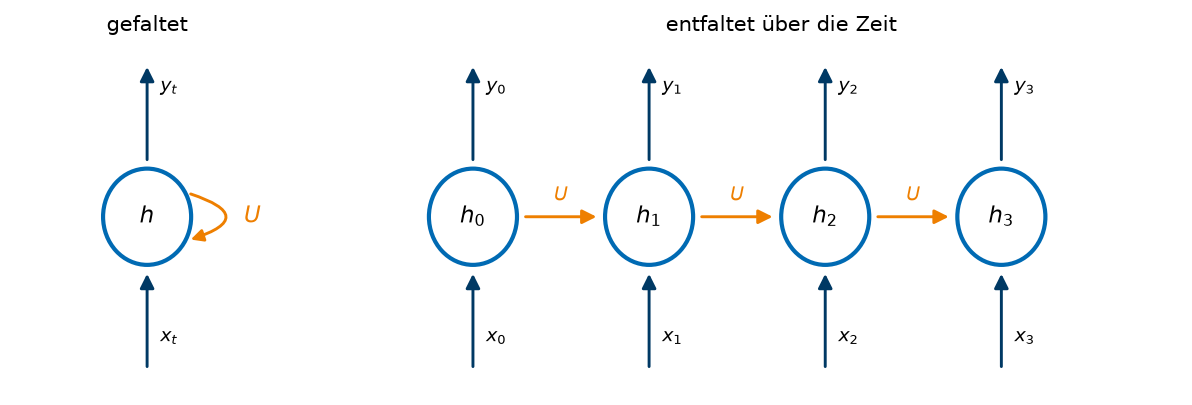
\includegraphics[width=0.78\textwidth]{vl09-rnn-unrolled.png}
  \end{center}

  \note{Über $T$ Zeitschritte entfaltet: ein Netz mit $T$ Schichten, die sich alle
    \emph{dieselben} Gewichte teilen. Backpropagation funktioniert dann ganz normal ---
    das heißt backpropagation through time.
    Und damit auch das bekannte Problem: Gradienten über viele Zeitschritte werden
    exponentiell klein oder groß.}
\end{frame}

\begin{frame}
  \frametitle{Skip Connections}

  \begin{center}
    \Huge $x^{(m)} = x^{(m-1)} + \operatorname{res}(x^{(m-1)})$
  \end{center}

  \bigskip
  \begin{center}
    \normalsize Jede Schicht ist nah an „nichts ändern“ ---\\
    und der Gradient hat einen Weg \emph{an} der Schicht vorbei.
  \end{center}

  \note{Auch Residual Connections genannt. Die Idee ist so einfach wie wirkungsvoll und
    steckt in RNNs, in ResNets (daher der Name) und in jedem Transformer-Block.
    Am Term $x^{(m-1)}$ sieht man es: Beim Ableiten bleibt eine 1 stehen, also kommt
    immer etwas durch.}
\end{frame}

\begin{frame}
  \frametitle{Gated RNNs}

  \begin{center}
    \Large
    \textbf{GRU}: Reset Gate, Update Gate\\[14pt]
    \textbf{LSTM}: hidden state $h_t$ \emph{und} cell state $c_t$,\\
    drei Gates: forget, input, output
  \end{center}

  \note{Die Gates sind Sigmoide mit Werten in $(0,1)$, die elementweise multiplizieren ---
    also genau die stetigen Bitmasken aus VL 7. Diesen Rückbezug machen, dann ist das
    nichts Neues mehr.
    Der cell state wird nur durch Addition und elementweise Multiplikation verändert:
    eine Skip Connection durch die Zeit.
    Schaltbilder gibt es auf Wikipedia (CC-BY-SA), im Skript verlinkt.}
\end{frame}

\begin{frame}[fragile]
  \frametitle{LSTM praktisch}

  \begin{lstlisting}
class MyModel(nn.Module):
    def __init__(self, embedding_length, hidden_size, output_size):
        super().__init__()
        self.lstm = nn.LSTM(embedding_length, hidden_size)
        self.label = nn.Linear(hidden_size, output_size)

    def forward(self, x):
        h, (h_n, c_n) = self.lstm(x)
        return self.label(h)
  \end{lstlisting}

  \note{\texttt{nn.LSTM} bekommt eine Sequenz von Vektoren (z.B. die word2vec-Embeddings
    aus der letzten Woche) und liefert die Sequenz der hidden states; darauf ein linearer
    Layer für die Vorhersage.
    $h_n$ und $c_n$ sind der \emph{letzte} Zustand --- für eine Klassifikation des ganzen
    Satzes würde man die nehmen.}
\end{frame}

\begin{frame}
  \frametitle{Geschichte in einer Zeile}

  \begin{center}
    \Large
    1982 Hopfield \; 1985 Boltzmann \; 1997 LSTM\\[10pt]
    2014 GRU \; 2017 Transformer
  \end{center}

  \note{Bill Gates 2018: „huge milestone in advancing artificial intelligence“ --- weil
    OpenAI mit LSTMs Dota 2 gewann. AlphaStar (StarCraft 2, 2019) war auch LSTM-basiert.
    Und dann kam etwas, das gar keine Rekurrenz mehr hat.}
\end{frame}

% ------------------------------------------------------------------ Transformer
\begin{frame}
  \frametitle{Wie misst man Übersetzungsqualität?}

  \begin{center}
    \Large BLEU (2001)
  \end{center}

  \bigskip
  \begin{center}
    \normalsize geometrisches Mittel der $n$-Gramm-Präzisionen,\\
    mal einem Strafterm für zu kurze Übersetzungen.
  \end{center}

  \note{„The closer a machine translation is to a professional human translation, the
    better it is.“ Menschliche Bewertung ist gut, aber teuer.
    Wichtig für die Einordnung: 41.8 „BLEU“ heißt 0,418. sacreBLEU ist die
    Standard-Implementierung. Und das WMT19-Modell aus VL 3 ist ein Nachfolger genau
    dieser Linie.
    Ohne so ein Maß hätte es das Paper von 2017 nicht gegeben --- man konnte plötzlich
    Architekturen vergleichen.}
\end{frame}

\begin{frame}
  \frametitle{2017: Attention is all you need}

  \begin{center}
    \Huge
    $\operatorname{Attention}(Q,K,V) = \operatorname{sm}\!\left(\dfrac{QK^T}{\sqrt{d_k}}\right)V$
  \end{center}

  \note{\textbf{Die Formel langsam lesen.} $Q$, $K$, $V$ sind lineare Projektionen der
    Token-Vektoren: Jedes Token \emph{fragt} mit seiner Query alle anderen, vergleicht mit
    deren Keys (Skalarprodukt!), macht daraus über Softmax Gewichte und sammelt eine
    gewichtete Summe der Values ein.
    Das Kochrezept aus VL 2 ist immer noch dasselbe: Skalarprodukt, dann etwas
    Nichtlineares.
    $\sqrt{d_k}$ ist Numerik --- ohne die Skalierung werden die Skalarprodukte in hohen
    Dimensionen zu groß und der Softmax zu spitz.}
\end{frame}

\begin{frame}
  \frametitle{Was ein Transformer-Block enthält}

  \begin{center}
    \Large
    Multi-Head Self-Attention\\[8pt]
    MLP\\[8pt]
    Residual Connections\\[8pt]
    Layer-Normalisierung
  \end{center}

  \note{Encoder-Stapel und Decoder-Stapel, beide aus identischen Blöcken dieser Bauart.
    Alles darin kennen wir schon --- Skalarprodukt, MLP, Skip Connections, Normalisierung.
    Neu ist nur, \emph{wer} mit \emph{wem} redet.
    Wer das Bild will: Figure 1 in Vaswani et al. Eine annotierte, ausführbare Fassung ist
    \emph{The Annotated Transformer}.}
\end{frame}

\begin{frame}
  \frametitle{Wo ist die Reihenfolge geblieben?}

  \begin{center}
    \Large
    Attention ist \emph{permutationsinvariant}.\\[16pt]
    Also: Positionskodierung addieren.
  \end{center}

  \note{Das ist die Frage, die man selbst stellen sollte, wenn sie nicht kommt: Wenn jedes
    Token mit jedem redet --- woher weiß das Modell, was vorne und hinten ist?
    Antwort: Jedes Token bekommt eine Positionskodierung addiert. Bei GPT ist sie gelernt,
    im Originalpaper sind es Sinus- und Kosinusfunktionen.}
\end{frame}

\begin{frame}
  \frametitle{GPT}

  \begin{center}
    \Large
    \emph{Decoder-only}: das nächste Token vorhersagen\\[12pt]
    self-supervised auf riesigen Textmengen\\[12pt]
    BPE als Tokenizer, gelernte Positionen, begrenzter Kontext
  \end{center}

  \note{Generative Pretrained Transformer. Varianten: GPT-2, GPT-J, GPT-NeoX, Llama.
    \emph{Self}-supervised ist der präzisere Begriff: Das Label ist das nächste Token,
    also steckt es schon in den Daten --- dieselbe Idee wie beim Autoencoder.
    Visualisierung Layer für Layer: bbycroft.net/llm --- das lohnt sich im Browser, wenn
    Zeit ist.}
\end{frame}

\begin{frame}
  \frametitle{Byte Pair Encoding}

  \begin{enumerate}\setlength{\itemsep}{8pt}
  \item Alle Tokenpaare nach Häufigkeit sortieren
  \item Das häufigste Paar zu einem neuen Token verschmelzen
  \item Wiederholen, bis das Vokabular groß genug ist
  \end{enumerate}

  \bigskip
  \begin{center}
    \normalsize GPT-4: 100\,256 Token, im Mittel etwa 4 Bytes pro Token.
  \end{center}

  \note{Das ist die Antwort auf die Tokenisierungsfrage aus der letzten Woche: nicht
    Wörter, nicht Zeichen, sondern ein \emph{flexibles} $n$. Häufige Wörter werden ein
    Token, seltene zerfallen in Silben oder Buchstaben.
    Die Idee ist von 1994 (Gage) und war ursprünglich ein Kompressionsalgorithmus.}
\end{frame}

\begin{frame}
  \frametitle{BERT}

  \begin{center}
    \Large
    \emph{Encoder-only}\\[12pt]
    Masked Language Modeling + nächster Satz\\[12pt]
    \normalsize Kontext in \emph{beide} Richtungen
  \end{center}

  \note{Masked Language Modeling ist word2vec mit Transformer --- die Lücke wird
    vorhergesagt, aber mit Kontext von links \emph{und} rechts. Deshalb das B für
    bidirectional.
    Bei gleicher Größe besser als GPT für Klassifikationsaufgaben; nicht zwangsläufig
    generativ.
    DistilBERT aus VL 3 ist genau davon die destillierte Variante.}
\end{frame}

\begin{frame}
  \frametitle{ViT: ein Bild als Satz}

  \begin{center}
    \Large
    Bild in Patches rastern\\[10pt]
    jeder Patch ist ein Token\\[10pt]
    2D-Positionskodierung
  \end{center}

  \bigskip
  \begin{center}
    \normalsize „An Image is Worth 16x16 Words“
  \end{center}

  \note{Ansonsten ein ganz normaler Transformer. Für Klassifikation manchmal besser als
    CNNs --- was die Frage aufwirft, wozu man CNNs noch braucht. Antwort nächste Woche.}
\end{frame}

\begin{frame}
  \frametitle{Vor der Winterpause}

  \begin{itemize}\setlength{\itemsep}{8pt}
  \item Das Übungsblatt (Faltung) hat bis \textbf{13.01.} Zeit
  \item Nutzen Sie die Pause als Pause
  \end{itemize}

  \bigskip
  \begin{center}
    Im Januar: Faltung und CNNs, dann LLMs praktisch.
  \end{center}

  \note{Ausdrücklich sagen, dass das Übungsblatt über die Winterpause läuft und niemand in den
    Ferien arbeiten muss.
    Die erste Übung im Januar ist eine Fragestunde --- Fragen dafür kann man vorab in der
    ILIAS-Umfrage sammeln, die dafür freigeschaltet ist.}
\end{frame}

\end{document}

%%% Local Variables:
%%% mode: latex
%%% TeX-master: t
%%% End:
